\section{Backup: how much of its window a model can use}
\label{sec:backup}

These builds sit after the last slide of the deck, out of the main sequence. The lecture shows them only when a student asks how much of its window a model can use.

\subsection{Effective length falls short of the window}
\label{sec:it-B-6-2}

\bi
\item \textbf{RULER} (Hsieh et al., 2024) asks how much of its window a model can use.
\item \textbf{The method:} synthetic tasks with more needles, tracing and aggregation.
\item \textbf{The effective length:} the longest tested length above Llama2-7B's 4K score.
\item \textbf{The reported result:} almost every model's effective length is below its claim.
\ei

Cheng-Ping Hsieh, Simeng Sun, Samuel Kriman, Shantanu Acharya, Dima Rekesh, Fei Jia, Yang Zhang and Boris Ginsburg (NVIDIA), RULER: What's the Real Context Size of Your Long-Context Language Models?, First Conference on Language Modeling (COLM 2024). We use arXiv:2404.06654 version 3 of August 6, 2024, the COLM version, which evaluates 17 models and keeps version 1's numbers for GPT-4, Yi (34B) and LWM (7B). The OpenReview record lists seven authors, without Yang Zhang. RULER is the companion to Lost in the Middle, and one of its needle tasks is that paper's key-value retrieval. On the map it sits in the evaluations lane.

The paper asks how much of its claimed window a model can use. Model releases of 2024, among them Gemini 1.5 and Claude 3, reported their long windows with the needle-in-a-haystack test, which Section 1 names beside passkey retrieval as the common synthetic tests. That test hides one fact, the needle, in long filler text, the haystack, and asks for it. The abstract calls it ``indicative of only a superficial form of long-context understanding''. GPT-4, Yi (34B) and LWM (7B) score 100.0 on it and on passkey retrieval at every length from 4K to 128K (Tables 10 and 11), so by these tests every window looks usable.

RULER keeps the needle test's control, synthetic text of a chosen length with a known answer, and makes the tasks harder. Its 13 tasks fall into four categories (Section 3). Retrieval keeps the single needle, with the passkey and vanilla needle tests among its eight tasks, and adds the needle among distractor needles and requests for several values or several keys. Multi-hop tracing follows a chain of variable bindings, X2 = X1, X3 = X2 and on, and returns every name bound to one value. Aggregation returns the most frequent words of a long list. Question answering hides the paragraphs that answer a SQuAD or HotpotQA question among other paragraphs. Each task runs at 4K, 8K, 16K, 32K, 64K and 128K tokens, and the score at a length is the mean accuracy over the 13 tasks (Section 4).

The effective length turns each curve into one number. The bar is 85.6, the 13-task mean of Llama2-7B (chat), a model with a 4K window, at 4K. The longest tested length whose mean exceeds the bar is the model's effective length, which Table 3 prints beside its claimed length (Section 4, ``Effective Context Size''). A long-context model therefore counts as effective at a length while it still beats a 7B model working at 4K. Table 3 grades only these six lengths, so it never grades a claim above 128K at the claim itself.

Every model in Table 3 except Gemini-1.5-Pro falls below the bar before its claimed length. Gemini-1.5-Pro stays above the bar at every tested length, 94.4 at 128K, and its 1M claim was not tested. Ten of the 17 models pass the bar at 32K, which the abstract reports as ``only half of them''. An et al. (Why Does the Effective Context Length of LLMs Fall Short?, ICLR 2025) trace the gap to training: relative positions far apart are rarely trained, and open models' effective lengths typically stay under half their training lengths. The next slide shows that the effective length also depends on the operation.

Every value in the chart is printed in version 3 of the paper: the needle scores in Table 11 (p. 24), and the 13-task means, the bar and the claimed and effective lengths in Table 3 (p. 7). None is read off a figure. The three models are three of the four that score 100.0 on the vanilla needle test at every length. The fourth, GLM4 (9B), is left out because its line would run beside GPT-4's. The lines join the six lengths of Tables 3 and 11, the only lengths they measure, and the accuracy axis starts at 60. RULER places the evidence at varied depths but reports one number per length, with no accuracy by position, the variable Lost in the Middle studies. The paper lists this first among its limitations (Section 8, ``Lack of position controlling''). In the second, the authors offer RULER as ``convenient behavioral checks'' that ``should not be preferred over more realistic settings''. The results describe models evaluated in 2024 on synthetic tasks, and a present model needs its own measurement.

\begin{figure}[htbp]
\centering
\includegraphics[width=\linewidth]{context/effective-length-5.png}
\caption{Effective length falls short of the window. The figure as it stands after the build's last click.}
\label{fig:effective-length-5}
\end{figure}

\paragraph{The figure, stage by stage.}
\be
\item The key lists three models evaluated in 2024 and the windows their makers claim: 128K tokens for GPT-4, 200K for Yi (34B) and 1M for LWM (7B). On the vanilla needle test, which hides one fact in filler text, all three score 100.0 at every length from 4K to 128K, the longest length of the paper's main tables (Tables 3, 10 and 11). By this test every window looks usable, and RULER asks how much of it each model can use.
\item The blue line is GPT-4 on RULER: the mean accuracy over 13 synthetic tasks with more needles, tracing and aggregation, the passkey and needle tests among them. Those two stay at 100.0, so the fall from 96.6 at 4K to 81.2 at 128K comes from the other eleven tasks. Strong simple retrieval coexists with a falling score on harder tasks.
\item The dashed bar is 85.6, the mean that Llama2-7B, a 7B model with a 4K window, scores at 4K. A model's effective length is the longest tested length whose mean exceeds the bar. GPT-4 scores 87.0 at 64K and 81.2 at 128K, so its effective length is 64K, half its claimed 128K. The ring marks that point.
\item Yi (34B) falls from 93.3 at 4K to 77.3 at 128K. Its last length above the bar is 32K, at 87.5, against a claimed 200K, beyond the six lengths of Table 3. Section 5 of the paper tests this model on single tasks up to 256K, its claim included, and analyzes its errors.
\item LWM (7B) starts at 82.3, already below the bar at 4K, and ends at 65.0. Table 3 prints its effective length as under 4K against a claimed 1M, although it scores 100.0 on the needle test at every length. The bullet that arrives with it states the result for all 17 models: almost every effective length is below the claim.
\ee

\begin{takeaway}The needle test overstates how much of a window a model can use.\end{takeaway}

\subsection{Effective length depends on the operation}
\label{sec:it-B-6-3}

\bi
\item \textbf{In the vending run,} a decision needs one fact, a chain of facts or a total.
\item \textbf{In RULER,} Llama3.1 (8B) is effective to 64K at finding, 8K at aggregating.
\item \textbf{In a harness,} each call should stay within its operations' effective lengths.
\ei

Hsieh et al., RULER, COLM 2024, as on the slide \hyperref[sec:it-B-6-2]{``Effective length falls short of the window.''} The figure adapts three of RULER's task categories to the vending log. Finding one fact is retrieval, following a chain of facts is multi-hop tracing, and combining many lines is aggregation. The decisions of the vending run need all three: the daily fee is one line, the due date of order 17 follows through shipment 5, and the units on order add up across five lines.

RULER also grades each category on its own, against Llama2-7B's 4K score on that category: 96.9 for retrieval, 89.7 for tracing and 84.8 for aggregation (Appendix F, Tables 13 to 15). On the 13-task mean, Llama3.1 (8B) is effective to 32K. By category, it is effective to 64K on retrieval and on tracing, and to 8K on aggregation, where its accuracy falls from 97.0 at 4K to 54.1 at 32K (Table 15). GLM4 (9B) and GradientAI/Llama3 (70B) also reach only 8K on aggregation. The order differs by model: GPT-4 is effective to 32K on retrieval, 128K on tracing and 64K on aggregation. One effective length per model therefore overstates the usable length for some operations and understates it for others.

The third bullet is the course's reasoning, and RULER evaluates no harness. The harnesses of the strategies segment compact as the window fills: Pi when the tokens in context exceed the window minus a reserve, 16384 tokens by default, and Claude Code as the window fills (the slides \hyperref[sec:it-7-5a]{``Pi compacts into a structured summary.''} and \hyperref[sec:it-7-5b]{``Claude Code summarizes and re-reads files.''}). A context that grows to the window can pass the length at which the operations a decision needs still work. Compaction helps in two ways. It keeps each call short, and a summary that records the resolved chain (order 17, due Day 4) or the running total (26 units ordered in all) turns a later trace or aggregate over a long log into a find over a short one. The summary step is itself an aggregation over the history, the category RULER offers as its proxy for summarization (Section 3.3), and aggregation fails first for Llama3.1 (8B), so the summarizer also needs an input it can use. RULER's numbers describe models evaluated in 2024 on synthetic tasks, so a run measures these lengths on its own model and operations.

The slide \hyperref[sec:it-10-2]{``Stress tests target what compaction can lose.''} reuses this test logic. It plants a commitment with a known answer in the run's history, compacts, and checks automatically that the next decision still has it.

The log lines, the highlighted lines and the three answers are illustrative. The rows adapt three of RULER's categories to a vending log: find stands for retrieval, trace for variable tracking, and aggregate for common-word and frequent-word extraction. Those two tasks count words, where the figure adds units. The figure draws no length and claims no score. RULER's fourth category, question answering, is left out. Its bar is 49.7, so its effective lengths come out long although its scores start lowest: at 4K, question answering is the lowest of the four categories for 16 of the 17 models (Tables 13 to 16). RULER generates its own synthetic inputs for each task at each length. The effective lengths of the second bullet are those of Tables 13 and 15, for a model evaluated in 2024.

\begin{figure}[htbp]
\centering
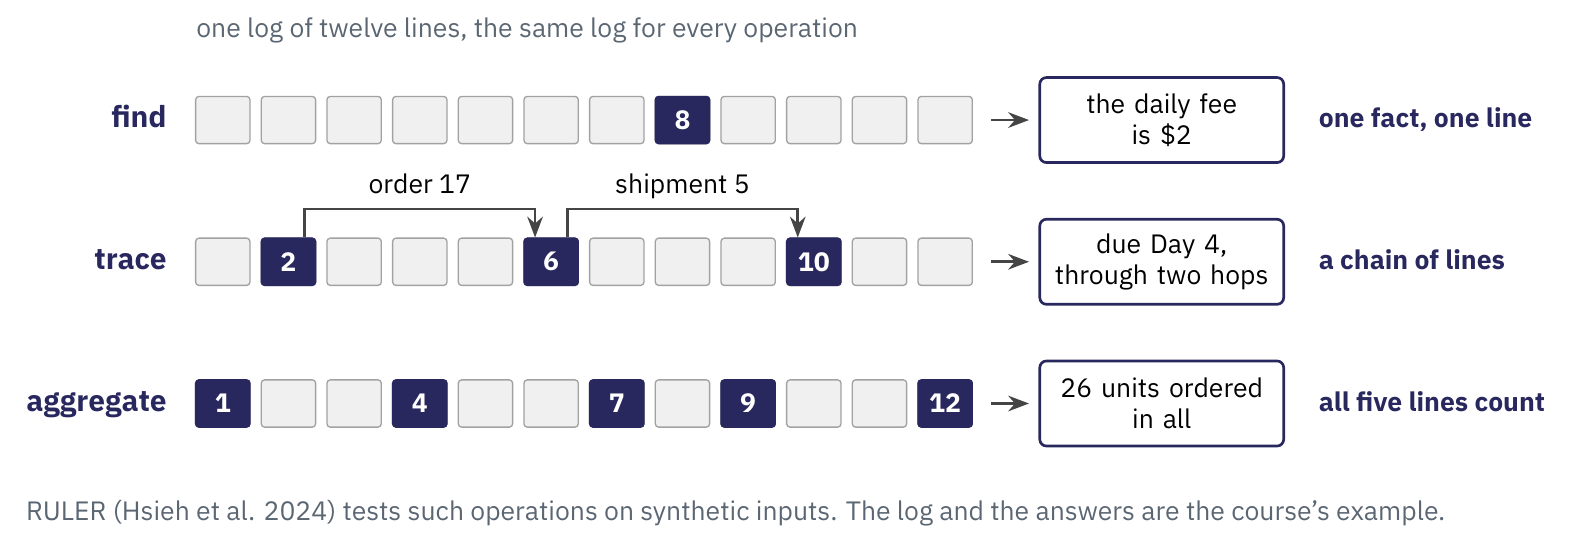
\includegraphics[width=\linewidth]{context/context-tasks-3.png}
\caption{Effective length depends on the operation. The figure as it stands after the build's last click.}
\label{fig:context-tasks-3}
\end{figure}

\paragraph{The figure, stage by stage.}
\be
\item Find: line 8 alone holds the answer, the daily fee is \$2, so the verdict reads one fact, one line. This is RULER's retrieval, the needle test and its harder variants, on the run's own log. Every later row reads the same log of twelve lines.
\item Trace: line 2 points to line 6 through order 17, and line 6 points to line 10 through shipment 5. The answer, due Day 4, through two hops, needs a chain of lines. RULER's variable tracking follows a chain of bindings in the same way: X2 = X1, X3 = X2 and on.
\item Aggregate: the answer, 26 units ordered in all, adds up lines 1, 4, 7, 9 and 12. All five lines count, so a model that misses any one of them returns a wrong total. The bullet that arrives with this row gives RULER's measurement for Llama3.1 (8B): effective to 64K at finding and to 8K at aggregating.
\ee

\begin{takeaway}A harness must test the operations its task needs at the lengths it expects.\end{takeaway}
